\chapter{Methodology}
\label{ch:methodology}

% \section{Overview}

% Explain what I want to do using the CMIP6 simulations: Describe what the general plan is: Visualization of the moisture transport in Europe with the help. 
% Also define what the goals of the visualizations are: Visualize different scenarios for comparison, visualize uncertainties of different members, visualize evolution over time, also try combining those. 
% Here should be a graphic that explains the workflow that transforms a simulation into some nice pictures
%
This Section gives a detailed description how the analysis was performed on the basis of the MPI GE CMIP6, how the huge datasets were preprocessed, the EOF computed and the result visualized. 

\section{Preprocessing}
\label{sec:preprocessing}

The purpose of this step is to prepare the datasets for generating the patterns via EOF and generating visualizations. For this the datasets need to be reduced to the area of interest (northern Atlantic and Europe), the directory structure shown in Figure~\ref{fig:data-structure} needs to be simplified, the necessary moisture transport (see Section~\ref{sec:moisture-transport}) needs to be calculated and data needs to be reduced to different time resolutions (daily, monthly). \todo{Still need to write somewhere why}

The calculations were performed on the high performance computing cluster\footnote{https://docs.dkrz.de/doc/levante/} of the German Climate Calculations Center (DKRZ), due to the MPI GE CMIP6 is saved there and downloading the data would take a lot of time. 
This also result in the goal of this step to minimize the hours on the HPC system since they get billed by the time using nodes. 
Although these steps seem easy, due to the large sizes of the datasets and other issues many challenges were met. 
In the following those will be explained with regard to the step they occurred in. 



\subsection{Chosen Framework}
\label{sec:preprocessing_framework}

The goal of this step is to prepare the data for further usage. 
After a few failed attempts with other languages/tools (CDO and Julia, see Section~\ref{sec:preprocessing challanges}), the Python libraries xarray \cite{hoyer_xarray_2017} and dask \cite{rocklin2015dask} were chosen as the fitting tools for this step.
Xarray is a library for handling n-dimensional, labeled arrays. It supports multiple input and output options (amongst others the required NetCDF format) and is compatible with the most popular scientific Python libraries (e.g. Pandas, NumPy). 
It comes with a great variety of features, making it easy to index and transform data and dimensions, joining different datasets (either along a dimension like time or multiple different variables having the same dimensions) and many more. 
But most important, it leverages the Dask library, which enables xarray to actually use the infrastructure of the DKRZ HPC cluster. 
Dask is enabling parallel and out-of-the-core\footnote{This usually means handling datasets larger than RAM, using disks (usually SSDs) as extension for RAM.} computing for the Scientific Python stack. 
Its goal is to be a NumPy clone leveraging the full potential of modern hardware, which usually utilizes multiple computing cores, without the need for rewriting the already existing scientific Python stack. 
It uses an acyclic task graph, which distributes tasks efficiently over multiple workers, which can be either different threads or processes. \cite{rocklin2015dask}


\subsection{Process}

The following the process for handling one timescope of member of one scenario is described. For one member the different timescope files are handled iteratively. 
Scaling it up for all the members is trivial by either running them in parallel on multiple nodes of the cluster (for the relatively computation-heavy IVT calculation) or by running different members iteratively (for simple variables). 
The high resolution of 6 hourly data is used at first for all the variables since it can be trivially reduced to daily/monthly means later. 

\textbf{1. Loading the Dataset}

In the first step the process is to load the required dataset(s) into xarray. 
This means not actually loading the grids into RAM but rather loading the metadata. 
The actual loading and computation is only performed when required (e.g. when writing the result), every step in between only returns another xarray (meta)dataset. 
Xarray offers different methods for either loading one dataset file or multiple, the latter is needed for the IVT calculation since multiple different variables need to be used. 
Important choices are here setting the \texttt{compat} parameter and choosing the chunking for Dask. 
The first one needs to be set to \textit{override}, which prevents xarray to check variables with the same label for compatibility (in this case here dimension like \textit{lon, lat, time} and the pressure fields \textit{ps}), which is useful e.g. when using dataset of different sources, but since all datasets conform to the same resolutions it is unnecessary. 

\begin{figure}[htb]
  \begin{center}
    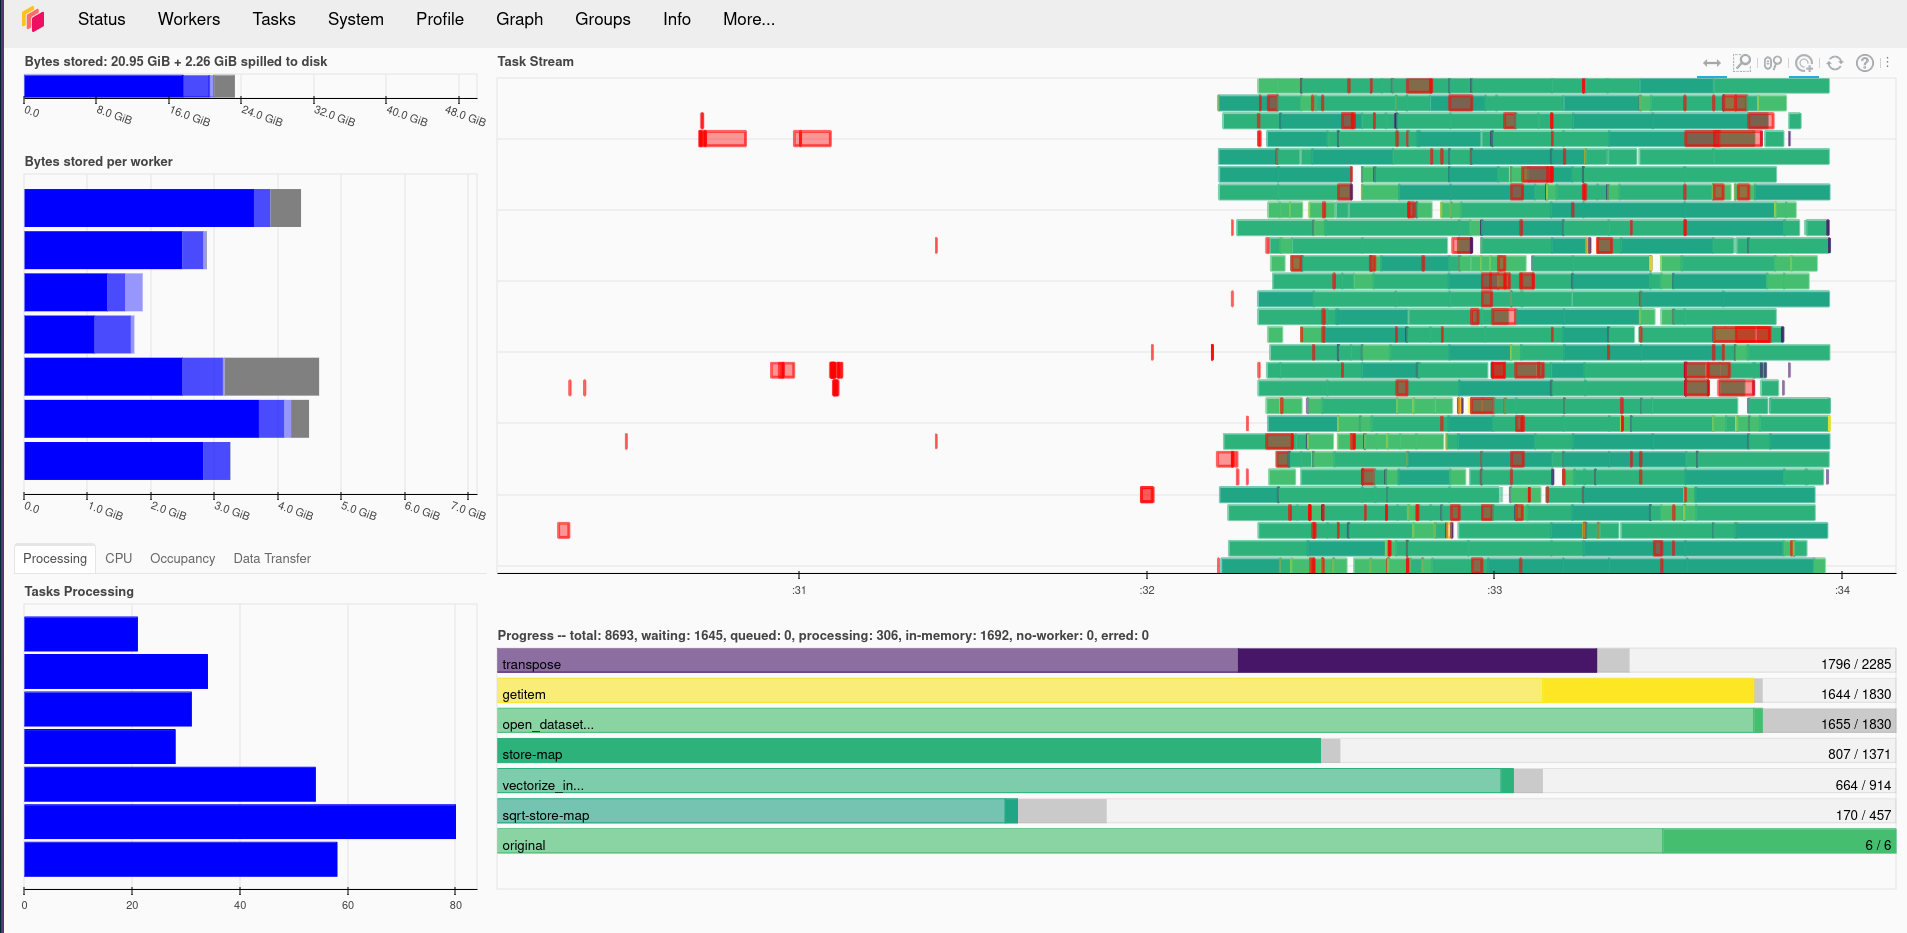
\includegraphics[width=0.95\textwidth]{figures/dask_dashboard_example.png}
  \end{center}
  \caption{Example of the general overview of the dask dashboard used for analyzing the efficiency of the process.}
  \label{fig:dask-dashboard}
\end{figure}


The latter choice is far more important:  
In NetCDF datasets data is often grouped into chunks of a certain, useful size and these chunks can then be compressed to reduce disk memory usage. 
If the chunks are compressed reading anything smaller than a chunk is useless, since the whole chunk needs to be loaded anyway to decompress it. 
Also reading too small chunks reduces the efficiency of dask, since the introduced scheduling overhead per task is too large and becomes overwhelming.
Furthermore, reading too small chunks result in too much worker-to-worker communication, which also results in significantly decreased execution time. 
On the other hand, reading too large chunks results in memory spills\footnote{This refers to a function in dask where overloaded workers save data on disk to prevent the worker from crashing} or workers crashing, which both significantly reduce execution time. 
To find the sweet spot of dask chunk size, dask offers a handy dashboard which visualizes the process of the dask task graph execution (see Figure~\ref{fig:dask-dashboard}). 
Grey areas in the \textit{Bytes stored per worker} section in Figure~\ref{fig:dask-dashboard} show memory spilled to disk, which is an indicator for too large chunk sizes. 
Red sections in the \textit{Task Stream} section refer to worker-to-worker communication, which may be an indicator for too small chunk sizes if they dominate the \textit{Task Stream}. 
So the Task overview given in Figure~\ref{fig:dask-dashboard} indicates a slightly too large chunk size, since too much is spilled to disk. \cite{buckley_choosing_nodate}

The chunk size in the available datasets is $(192, 96, 47, 1)$\footnote{\label{vardims}Referring to $(lon, lat, lev, time)$}, which means one chunk corresponds to one time snapshot of the whole atmosphere.
Following the previous argumentation, the only useful way of changing the chunks are different amounts of time snapshots per chunk.
Using the dask dashboard to evaluate different chunk sizes, the optimal chunk size with minimal spilled memory, worker communication and no crashing workers\footnote{For one of the DKRZ HPC cluster's nodes with 100 GB RAM} was $(192, 96, 47, 128)$\cref{vardims}.  


\textbf{2. Reduction to Area of Interest}

The next step is to cut out the geographical area of interest, which is the northern Atlantic and Europe. 
Following \cite{vietinghoff_visual_2021} and \cite{hurrell_overview_2003}, it was defined as $90^\circ W - 40^\circ E$, $20^\circ - 80^\circ N$.
Unfortunately for this case, the longitude coordinate is saved in the range of $[0,360]^\circ$, so it can't be loaded as one slice. 
Therefor, the longitude coordinates are first transformed to the form $[-180, 180]^\circ$, with negative values being $^\circ W$ and positive values being $^\circ E$. 
Then the area of interest can be cut out without problems and the result can either be used for further calculations (Step 3) or directly saved as a NetCDF file (Step 4). 

The size of data could be further reduced in this timestep by selecting only the relevant winter months (see Section~\ref{sec:eof_calc}), but with future work in mind the whole year was kept in this stage. 

\textbf{3. Calculating IVT Field}

The first step to calculate the IVT field is to convert the hybrid sigma pressure levels (see Section \ref{sec:hybridsigma}) to actual pressure values. 
For this Equation \ref{eq:mpige-sigma-hybrid-pressure} is used for calculating a new variable \texttt{plev} containing the pressure values at each grid point in each time step. 
Then NumPy's trapezoidal integration function is used to calculate the zonal (Equation \ref{eq:zonal_ivt}) and meridional (Equation \ref{eq:meridional_ivt}) components of the IVT. 
Similar to related literature \cite{ayantobo_integrated_2022}, a constant value for the gravitational acceleration $g = 9.806~ms^{-2}$ is used in the calculation. 
Using the result of the zonal and meridional components, the norm field $\lVert IVT \rVert$ can be calculated using Equation \ref{eq:ivtnorm}. 



\textbf{4. Saving Results to NetCDF dataset}

The results of these calculations (or the geographical box cutout) are then again saved as NetCDF files, in the far less complex directory structure \texttt{time\_resolution}, \texttt{variable}, \texttt{member} and then the actual file \texttt{timescope.nc}. 
In case of the IVT, both (zonal and meridional) components are saved alongside the Euclidean norm. 


\textbf{5. Generating daily/monthly means}

Since the related literature does not entirely agree regarding the timely resolution of IVT in EOFs (see Table \ref{tab:ivtpatterns-overview}), the six hourly data is reduced to monthly and daily means using CDO.
Monthly IVT is also called stationary moisture transport and dominates the total water vapor transport \cite{zhou_atmospheric_2005}, while the anomalies (departures from monthly mean per daily/subdaily timestep) are transient components.
Both are important parts of total moisture transport, but since a comparison of stationary and transient components is beyond the scope of this thesis, only monthly data will be used for the further analysis. 
The higher resolutions are still saved and can be used in future work. 

\subsection{Challenges of Preprocessing}
\label{sec:preprocessing challanges}

The steps described in the section before were just the final attempt. 
The first idea was using Climate Data Operators \cite{schulzweida2024}, a command line tool containing multiple operators for processing climate and similar data. 
The operators consist of common statistical and mathematical functions (mean, add, sum), sampling and data selection tools (select geographical or time limits) and other helpful operators like interpolations and even EOF calculation. 
Although this sounded very promising, it quickly turned out to be very complicated to implement the desired vertical integration in CDO.
The following idea was to implement the IVT calculation in Julia \cite{gao_julia_2020}, using just a NetCDF library \cite{barth_ncdatasetsjl_2024} while the rest was coded from scratch. 
The algorithm was very simple: 

\begin{enumerate}[itemsep=0mm]
  \item Load all datasets into the RAM (as recommended by the NetCDF library itself) and cut out the used geographical limits. This should be feasible since all in all one dataset for one timescope-file accounts for $\sim 12~GB$\footnote{$70~lon * 32~lat * 47~levels * 29220~timesteps * 4~byte \approx 12 GB$}, so the maximum is around $36~GB$, since the surface pressure data is not that large ($\sim 260~MB$)   
  \item Calculate the IVT with trapezoidial integration multithreaded by handling one time\-step by one thread
  \item Write the results (Euclidean norm and the meridional/zonal component)
\end{enumerate}

Although Julia promises high performance, it performed quite poorly on the HPC.
The reason for this is the slow IO on the cluster: While the calculation itself took only $\sim 235~s$ ($\approx 4~min$)\footnote{Referring here and  in the following to one timescope of 20 years in one member}, the loading of the required datasets took around $\sim 3350~s$ ($\approx 55~min$). 
This results in roughly $5 h$ (including saving the data to disk) for one member of ScenarioMIP, which leads to $250~h$ node hours for one scenario. 
Taking into account that it needs to run for historical simulations as well as other scenarios, this was not feasible according to the limited node hours provided\footnote{Also taking into account that the processes may need to run multiple times due to errors}.

To reduce the loading time of the data multiple optimizations were evaluated. 
First, the amount of moved data in memory was minimized by preallocating the needed RAM and writing directly to the preallocated space. 
Furthermore, other NetCDF libraries were tested, but simple loading times were very similar. 
Although this significantly reduced the amount of allocations, the effect on loading time was negligible. 
To actually archive a significant boost in loading time it was tried to load the required datasets (located in different files) in parallel. 
Unfortunately, the used library \cite{barth_ncdatasetsjl_2024} encountered a segmentation fault used in multiple threads, so the alternative libraries NetCDF.jl and HDF5.jl were explored, since the HDF5 standard allows parrallel access to files \cite{folk_overview_2011}. 
Although the parallel access to files using multiple threads (with HDF5.jl) lead to increased speeds in tests, the results did not yield any significant increased efficiency on the cluster itself.
Even splitting up the loading according to the chunking in the files (all data from one timestep is one chunk) and loading each timestep separately in one thread even increased the data loading time quite far.  
The next approach was to split the task up into different processes, each one loading data from one variable. This actually reduced time spent to one third in tests, but testing it on the actual data sizes revealed that the $12~GB$ are too much to be returned from the child processes loading the file to the mother process. 

From here on some other approaches could have been explored, like splitting up different time steps amongst different processes, but the far more suitable method of using xarray and dask has been found and implemented.


\section{EOF Calculation}
\label{sec:eof_calc}

In the next step, the patterns are calculated using Empirical Orthogonal Functions. While Section~\ref{sec:eof} gives the theoretical mathematical background, this Section describes the practical implementation, the sliding window approach and domain-specific challenges of calculating EOFs for different variables. The following description is for one member of the different scenarios, but is handled the same way for every member.  

This step was implemented in the Julia programming language \cite{bezanson_julia_2017}.
Although it was tried using it for the preprocessing and failed (see Section~\ref{sec:preprocessing challanges}), the reduction of the data was enough to make it easy working with  the NetCDF library  \cite{barth_ncdatasetsjl_2024} implemented in Julia. 
Julia has the advantage of making it particularly easy and intuitive working with matrices and high dimensional arrays. 
Additionally, it is (usually) also very computationally efficient doing so, which is the reason it was chosen for the implementation of this step. 
Other factors are the great reproducibility of code and the fact the Makie framework (based on Julia) was chosen for the visual analysis step (see Section~\ref{sec:vis_analysis}), which made it possible to reuse some already written code. 


In general, the procedure of this step is based on the approach of \cite{vietinghoff_visual_2021}, but has differences in a few places. 

% \subsection{EOF Calculation of one Time Window}

\textbf{1. Preparation of the Datasets for Sliding Window Approach}

In the very first step, the monthly data in form of multiple NetCDF files containing different time scopes are loaded. 
Since the influence of the NAO especially significant in the boreal winter, this thesis focuses on the extended winter season like \cite{vietinghoff_visual_2021}, keeping only the months December, January, February and March (in the following DJFM). 
So during loading the irrelevant months are filtered out, additionally to filtering out double values of months (a result of the monthly mean process with CDO), resulting in a timeline containing exactly one spatial map for each month value for each month. 
The data is now available in the form of a three-dimensional array with the shape $(lon, lat, time)$, while longitude, latitude and time are stored separately as one-dimensional arrays. 
To make changes from the (pre)industrial time to future scenarios visible, each scenario is concatenated with the historical simulation. 
Then the data is grouped in certain scopes for the sliding window approach. 
For this the data is grouped into winter seasons, one season is defined as a slice of data before a huge time threshold (e.g. 150 days, representing the spring/summer/autumn gap) to the next date. 
Following the argumentation of \citeauthorwork{vietinghoff_visual_2021}, the window size affects the smoothing of the data: The larger the time window, the better the noise is smoothed out.
But as a drawback small scale features are smoothed out along the noise. 
But since the focus of this thesis is monthly mean data, we are interested in the large scale structure of IVT and its connection to other variables, so rather large windows of 30 and 50 years were chosen, similar to \citeauthorwork{vietinghoff_visual_2021}.  
Similar to \citeauthor{vietinghoff_visual_2021}, scopes of 30 and 50 winters are implemented.  
The next scope is then shifted by one winter season, and again counted for 30/50 seasons. 
In difference to \cite{vietinghoff_visual_2021}, the winters themselves are not reduced to one mean map since this has not been done by any related work using IVT fields, and smoothing out the data any further could potentially remove important features. 


From here on steps are described for one time window of any variable. 
These steps are then computed the same for any other time scope of any member of any variable. 



\textbf{1. Preparation of the Data for SVD}

Before calculating SVD, the data needs to be prepared accordingly. 
After the scoping, the data for each scope is available as a 
Following the argumentation from \cite{vietinghoffdiss} and Section~\ref{sec:eof} the first step is to multiply each datapoint with the factor $\sqrt{m-1}^{-1}$\footnote{\label{timesize}$m$ being the time dimension size}. 
Then the geographical weights are applied, shifting the data into weighted space. 
The geographical weights are applied depending on the latitude of the data, approximated by $\cos(lat)$. 
Next, the data needs to be reshaped, since SVD only works for matrices (two-dimensional arrays): The geographical dimensions $(lon, lat)$ are reduced to one spatial dimension and then permuted, so the time is the first dimension. 
Now the shape of the data is $(time, spat)$, and SVD can be calculated. 

\textbf{2. Calculating EOFs with SVD}

In the next step the Singular Value Decomposition is applied to the geographically weighted two-dimensional data chunk. 
For this the SVD implementation of Julia's \texttt{Linear\-Algebra} package (which is part of the Standard Library) is used.
This approach computes all $m$\cref{timesize} modes, although at most the top five modes are used in this thesis. 
This was feasible for the monthly data used in this thesis, but once this approach is scaled up to daily or subdaily data it should be replaced by faster algorithms like Snapshot POD or the SLEPC implementation used by \citeauthor{vietinghoffdiss} \cite{vietinghoffdiss}.
Those implementations compute only the first $n$ modes, which is significantly faster than the full SVD computation. 

The result of the SVD of the weighted data chunk $D$ is then:

\begin{equation}
\label{eq:SVD}
L,S,R = SVD(D)
\end{equation}

$L$ are the left singular vectors, $R$ the right singular vectors and $S$ a vector containing the singular values. 
With time being the first dimension as a result of the previous step, $R$ contains the spatial modes, $L$ the temporal modes (also called principal components or EOF coefficients). 
The singular values $\Sigma$ can be used to compute the eigenvalues ($\sigma_i^2$), which are  the share of variability encoded in that corresponding mode $i$ with Equation~\ref{eq:eof variance calculation}. 
Then the modes are cut of at a limit $n$ (usually five) to reduce disk space usage and loading times in the visualization processes later. 


\textbf{3. Post Processing of the EOFs}

After the first $n$ modes of interest were cut off, a few more steps are required to be able to reconstruct the anomaly map generated in the preparation step.  
First, the temporal modes are scaled with $\sqrt{m-1}$, then the modes are aligned to some vector (see Section~\ref{sec:mode_alignment}) and the weighting is reverted by multiplying the spatial modes depending on their latitude with $\cos(lat)^{-1}$.
The results are then saved using a data structure serialization library called \texttt{JLD2}, which is based on HDF5 \cite{noauthor_juliaiojld2jl_2024}. 
For this the five most significant modes of the spatial and temporal patterns are persisted, alongside the singular values (for scaling and variability computation) and the sum of all eigenvalues
As stated in Section~\ref{sec:eof}, the spatial as well as the temporal patterns from the SVD are in unit scale, and since they are eigenvectors, any combination of a scalar $c$ and the EOF modes $cg^{(k)}$ and their corresponding temporal pattern $\alpha^{(j)}_k c^{-1}$ are also viable solutions to the problem. 
This leaves room for the scaling and choosing the sign of the spatial/temporal patterns in a way that simplifies interpretation of the patterns. 
The former is explained in Section~\ref{sec:mode_scaling}, the latter  in Section~\ref{sec:mode_alignment}.

\subsection{EOF Mode Scaling}
\label{sec:mode_scaling}

As explained by \citeauthorwork{vietinghoffdiss}, there are two particularly useful ways of scaling the results: 
Either by multiplying the temporal patterns (or here: the left singular vectors) with their corresponding singular value $\sigma_i$, which yields EOF coefficients in the original unit of measurement, or by multiplying the spatial pattern (or right singular vectors) with their corresponding singular value $\sigma_i$, which yields EOFs in the original unit of measurement. 
Depending on the type of used visualization, the former or latter are more fitting, so in contrast to \cite{vietinghoffdiss}, the scaling is done at the loading of the data to be more flexible.

\subsection{EOF Mode Alignment}
\label{sec:mode_alignment}

Since basically only two scaling modes are useful (see Section~\ref{sec:mode_scaling}), the sign/direction of that vector is a last, but very important choice to make.
While there is no inherent meaning in the sign of one certain pattern, it is crucial for understandability to align the results to a) compare modes across time and members and b) analyzing spatial and temporal patterns separated from each other. 
Most of the related work in Section~\ref{sec:related_pattern_analysis} uses maximum of a few modes (since most don't compute multiple modes, and none use an ensemble scale simulation), which enables them to align the modes by hand to be useful or don't align them at all.
Since this work has many more patterns to align for one scenario, it's not feasible to do it by hand, the problem needs to be solved algorithmically. 
The only work using such a large scale analysis is by \citeauthor{vietinghoffdiss} \cite{vietinghoffdiss}.  
Its solution for this is providing a field $F$ to which we compare our spatial mode and decide to whether flip it ($\equiv$ multiplying it with $-1$) or not. 

The method chosen by \citeauthor{vietinghoffdiss} \cite{vietinghoffdiss} is to use the Scalar/Dot product of the spatial pattern with the mean field used to generate the anomaly maps in the data preparation step. 
This mean field is then adjusted by the spatial mean, to reduce it to the actual values of variance. 
If the result of the scalar product is less than zero, meaning the spatial pattern is closer to the mean of the data. 
This process is illustrated in the Figure TODO \todo{Make fig with the mean fields, cleaned by spatial mean and the first EOF pattern} 
This has the effect that positive values of patterns align with above-average values of the actual data mean and vice versa, making the sign of the EOFs interpretable \cite{vietinghoffdiss} (see Figure TODO). 

Unfortunately, this works only well for the primary EOF mode, while the rest compared to yields not so successful results. 
A way of testing the alignment of patterns is by computing the cross-correlation boxplots from Section~\ref{sec:Temporal Pattern Correlation} with and without absolute correlation values.
Figure~\ref{fig:TODO} gives an example of such an analysis. 
If the absolute correlation boxplot shows a clear trend (e.g. consistent values) but the plot with normal correlation values has either no visible correlation (meaning the alignment is very arbitrary and varies a lot) or there are many outliers on the opposite side of the zero line (alignment did not work for just some members). 
To fix these problems and also measure correlation of the secondary or lesser modes, the spatial pattern of the first scope in the historical simulation is used as the field to align to as the best effort approach. Depending on the mode and variable this was more or less successful. 
The top five spatial patterns of each relevant variable (IVT, surface pressure and precipitation) are shown in Figure~\ref{fig:5modes each variable}.



\section{Analysis of EOF Patterns}
\label{sec:vis_analysis}

After generating and storing the EOF results, they can be used for analysis. 
This section contains the techniques and reasoning for decisions, while Chapter~\ref{ch:results} contains the descriptions and analysis of the full results. 
This section also takes reference to techniques used in related work. 

For this task Julia's Makie Framework \cite{danisch_makiejl_2021} was chosen. 
It allows to easily create a complex layout for figures and allows creating animations as well as interactive visualizations. 
It was made to \enquote{create high-performance, GPU-powered, interactive visualizations, as well as publication-quality vector graphics with one unified interface} \cite{danisch_makiejl_2021}. 
Additionally, there is a library\footnote{GeoMakie.jl: \url{https://geo.makie.org/}} available for projecting data onto different map projections. 


While the previous two Sections had the goal of generating the spatio-temporal EOF patterns (\textbf{M1} from Section~\ref{sec:research_questions}), this Section has the goal of fulfilling the other two milestones:  
Studying the relationships with other variables (\textbf{M2}) to get a sense of the meaning of the IVT EOF patterns as well as displaying the variability introduced by the multiple members of the chosen dataset (\textbf{M3}). 

% \subsection{Mode Reconstruction} % (fold)
% \label{sec:Mode Reconstruction}
%
% \todo{Evaluate whether this section is actually useful}
%
% This analysis uses EOF's ability of reconstructing the original data with a subset of modes.  
% The goal of this visualization is not to analyze the whole timeline, let alone the whole ensemble, but rather explaining what the EOF actually does and how certain modes contribute to the actual data. 
%
% The reconstruction is pretty straight forward, basically the steps taken in Section~\ref{sec:eof_calc} need to be reversed to reconstruct the data: 
% First the spatial patterns need to be reshaped to a two-dimensional matrix, then the approximated reconstruction of the original anomaly maps $\hat{D}$ is given as 
%
% \begin{equation}
%   \hat{D} = \hat{L} \cdot \hat{S} \cdot \hat{R}'
%   \label{eq:eof reconstruction}
% \end{equation}
%
% with $\hat{L}$ being the remaining temporal patterns, $\hat{S}$ the singular values, and $\hat{R}'$ the transposed, reshaped spatial modes. 
% Additionally, the original mean of the EOF scope can be added to the anomaly maps, resulting in an approximation of the actual data. 
%
% To help to understand before unknown patterns, it is useful to depict better understood patterns (i.e. patterns of Sea Level Pressure) next to other, rather unknown patterns (like IVT patterns) to maybe get insight about possible correlations and the original data. 
% To get insight about specific events, the generation function allows passing a filter function searching for certain values of the temporal patterns, e.g. looking for months when a certain pattern was particularly positively (or negatively) active, or not active at all. 
% The result can then either be presented as a visual analysis tool with a slider or as a video which can easily be shared.

% subsubsection Mode Reconstruction (end)

\subsection{Spatial Pattern Analysis}
\label{sec:mode comparison}


\begin{figure}[htb]
  \begin{center}
    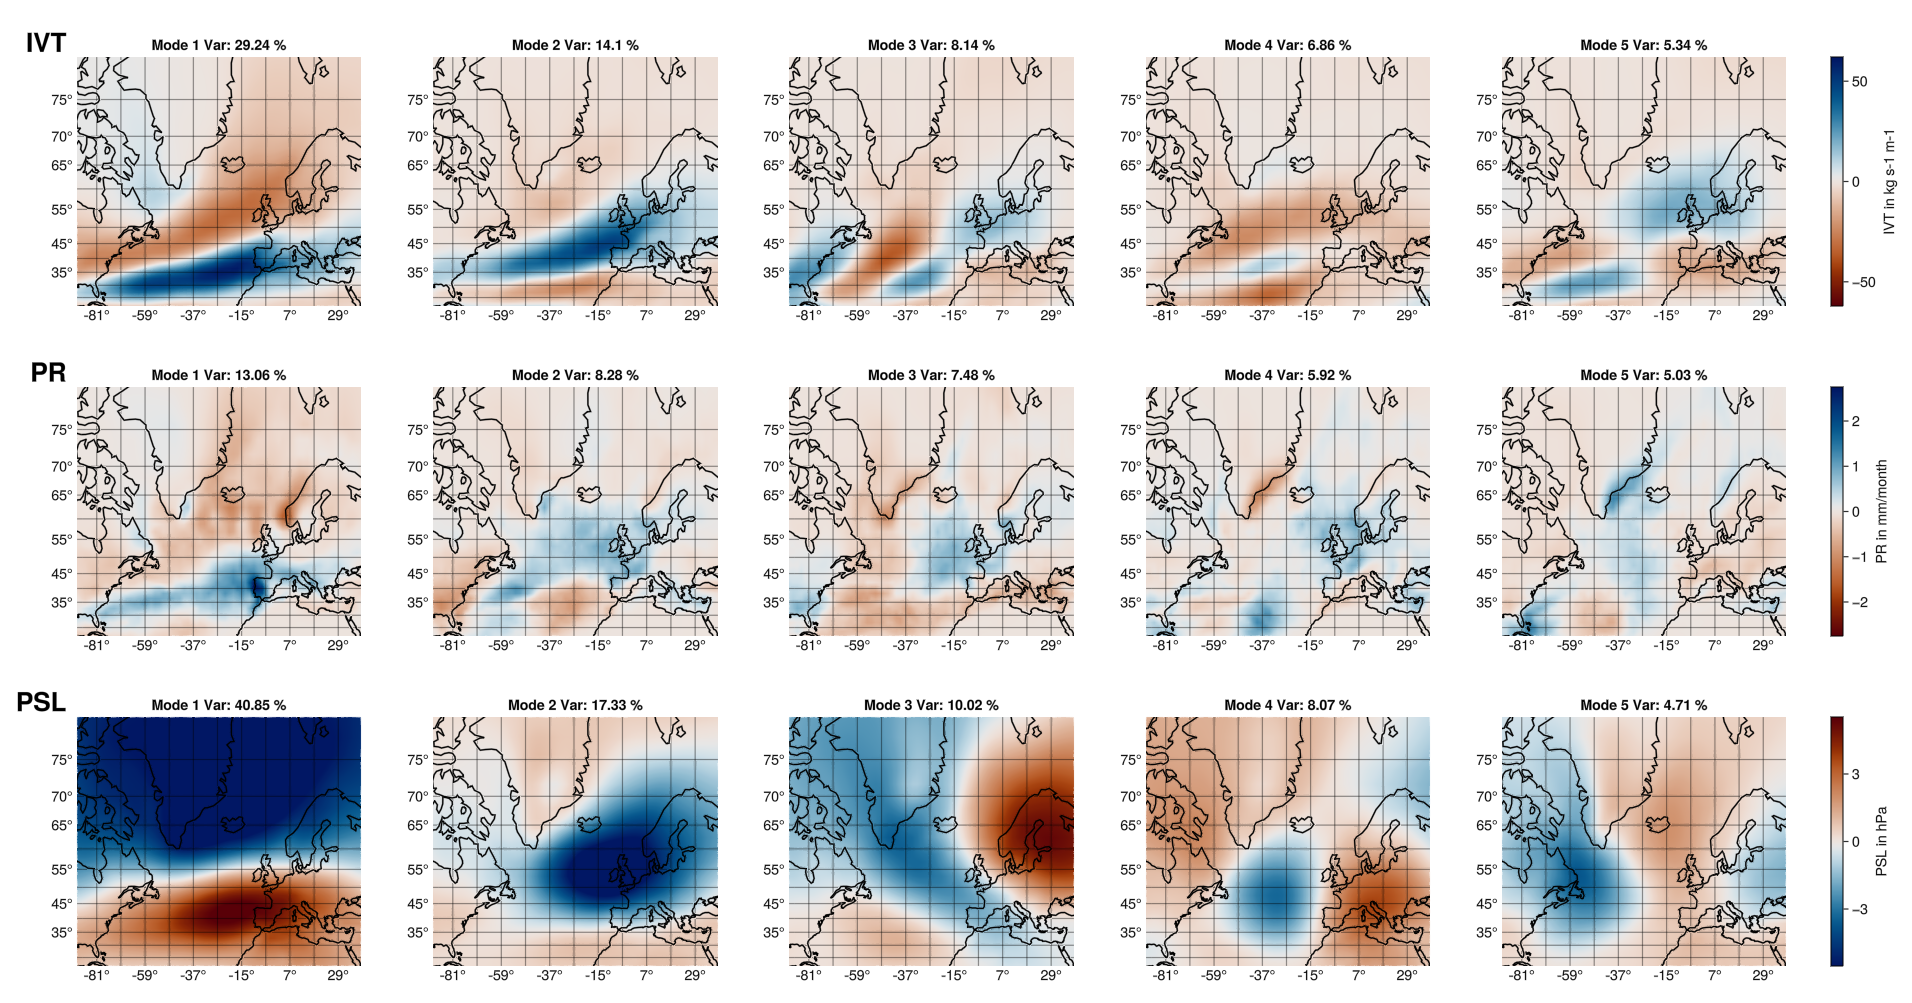
\includegraphics[width=0.95\textwidth]{figures/top5_spatial_modes_ivt_psl_pr_mem11_scope20.png}
\end{center}
  \caption{The five most significant modes of each of the processed variables (using the short names given in Table~\ref{tab:thesisVariables}). Taken from one member with 50 winter timescope and the scope from 1868 to 1918}
  \label{fig:5modes each variable}
\end{figure}


The main focus of this thesis lies in the visualization of the spatial patterns, since those are easy to understand visually.  
The main challenges are here to visualize the evolution of the pattern over time while still encoding the variability originating from the 50 members of the MPI GE CMIP6. 
Of course just one member could be used, or the data can be reduced to averages, but this also means losing the advantages of multiple member simulations. 
Although there are some examples of visualizing uncertainty in scalar fields (or features thereof like iso contours), none of them provide an existing implementation, which greatly hinders the usability. 
Since a new implementation of those concepts was outside the scope of this thesis, a new way of visualizing the ambiguity of multiple members needed to be found. 
While ways of representing uncertain scalar fields exist (like \cite{coninx_visualization_2011}), it may not always be helpful to visualize the full ambiguity of the dataset since it could generate too much visual clutter. 
Instead, a certain feature could be extracted to show the ensembles' variability.



\subsubsection{Feature Selection}

As shown in Section~\ref{sec:uncertainity_vis}, there exist multiple ways of visualizing scalar fields, either by transforming the actual scalar field somehow (like the approach of \citeauthorwork{coninx_visualization_2011}) or by selecting an interesting feature in it and visualizing it. 
The latter approach was used by  \citeauthorwork{vietinghoffdiss} (using the extreme points of the fields) and by \cite{sanyal_noodles_2010, whitaker_contour_2013} using contour lines.  

After analyzing the different spatial patterns of the different variables (and especially IVT), it was obvious that the separation line between the positive and negative spatial patterns seems to be very pronounced, especially in the primary modes. 
Therefor, the use of contour lines seemed like a good choice for a feature. 
Contour lines (also referred to as isolines) are lines, that share the same value of the function defining the field. The best known contour lines are lines of same height in maps of mountains.  
And since one question of the introduction was how those spatial patterns shift geographically, the contour line of zero, representing the borders of positive and negative patterns seems fitting. 
This procedure relates to the idea of level crossing probabilities, similar to the work of \citeauthorwork{poethkow_approximate_2013}, but for isolines and not for isosurfaces.

\subsubsection{Visualizing the Feature}

The most straight forward way of visualizing uncertain isolines are spaghetti plots as used in the work of \citeauthorwork{sanyal_noodles_2010}, by simply drawing all the isolines of the different members, usually in different colors. 
This was also implemented in this Thesis, but spaghetti plots have a lot of usual drawbacks. 
While they work very well for areas where the contour lines are very close to each other (see Figure~\ref{fig:TODO}), they tend to overcrawded areas making the visualization overwhelming and chaotic. 
Additionally, contour lines give a false sense of precision in data that is actually not that precise. 

\subsubsection{Level Crossing Probabilities using Hexbins}

To fix those issues of spaghetti plots, another method was implemented using hexbins. 
Hexbin plots\footnote{\url{https://docs.makie.org/dev/reference/plots/hexbin}} as used by \citeauthorwork{carr_hexagon_1992} for geographic data are an alternative to heatmaps, depicting the density of observations (usually given as points in space). 
Heatmaps divide the observed grid into rectangular areas of variable size, and colors the rectangular area depending on the number of observations in it. 
Hexbin plots are very similar, except they divide the grid into hexagonal \enquote{bins} and handle the observations in the same way as heatmaps. 
The advantage of hexbin plots is that it represents distribution better than square bins ($\equiv$ heatmaps) as it was depicted in \cite{carr_hexagon_1992}, as well that it can be more visually appealing to humans \cite{carr_hexagon_1992}. 
The main idea for this was to avoid the problems of the most straightforward way of displaying uncertain contour lines: spaghetti plots. 
While they work quite good when the results of all members align well and do not differ that much, they quickly get chaotic once that is not the case. 
This also scales with the number of members in the ensemble. 
A spaghetti plot with 10 members may look fine, but looks quite chaotic with 30. 
Once members are not easily countable anymore, it's hard to instinctively differentiate between a quite uncertain area (10 out of 50 members) and a quite likeable area (25 out of 50 members). 
To reduce this and make likely and make it possible to instantaneously evaluate how likely an area is to contain isolines, the hexbin approach was explored.


\begin{figure}
  \begin{center}
    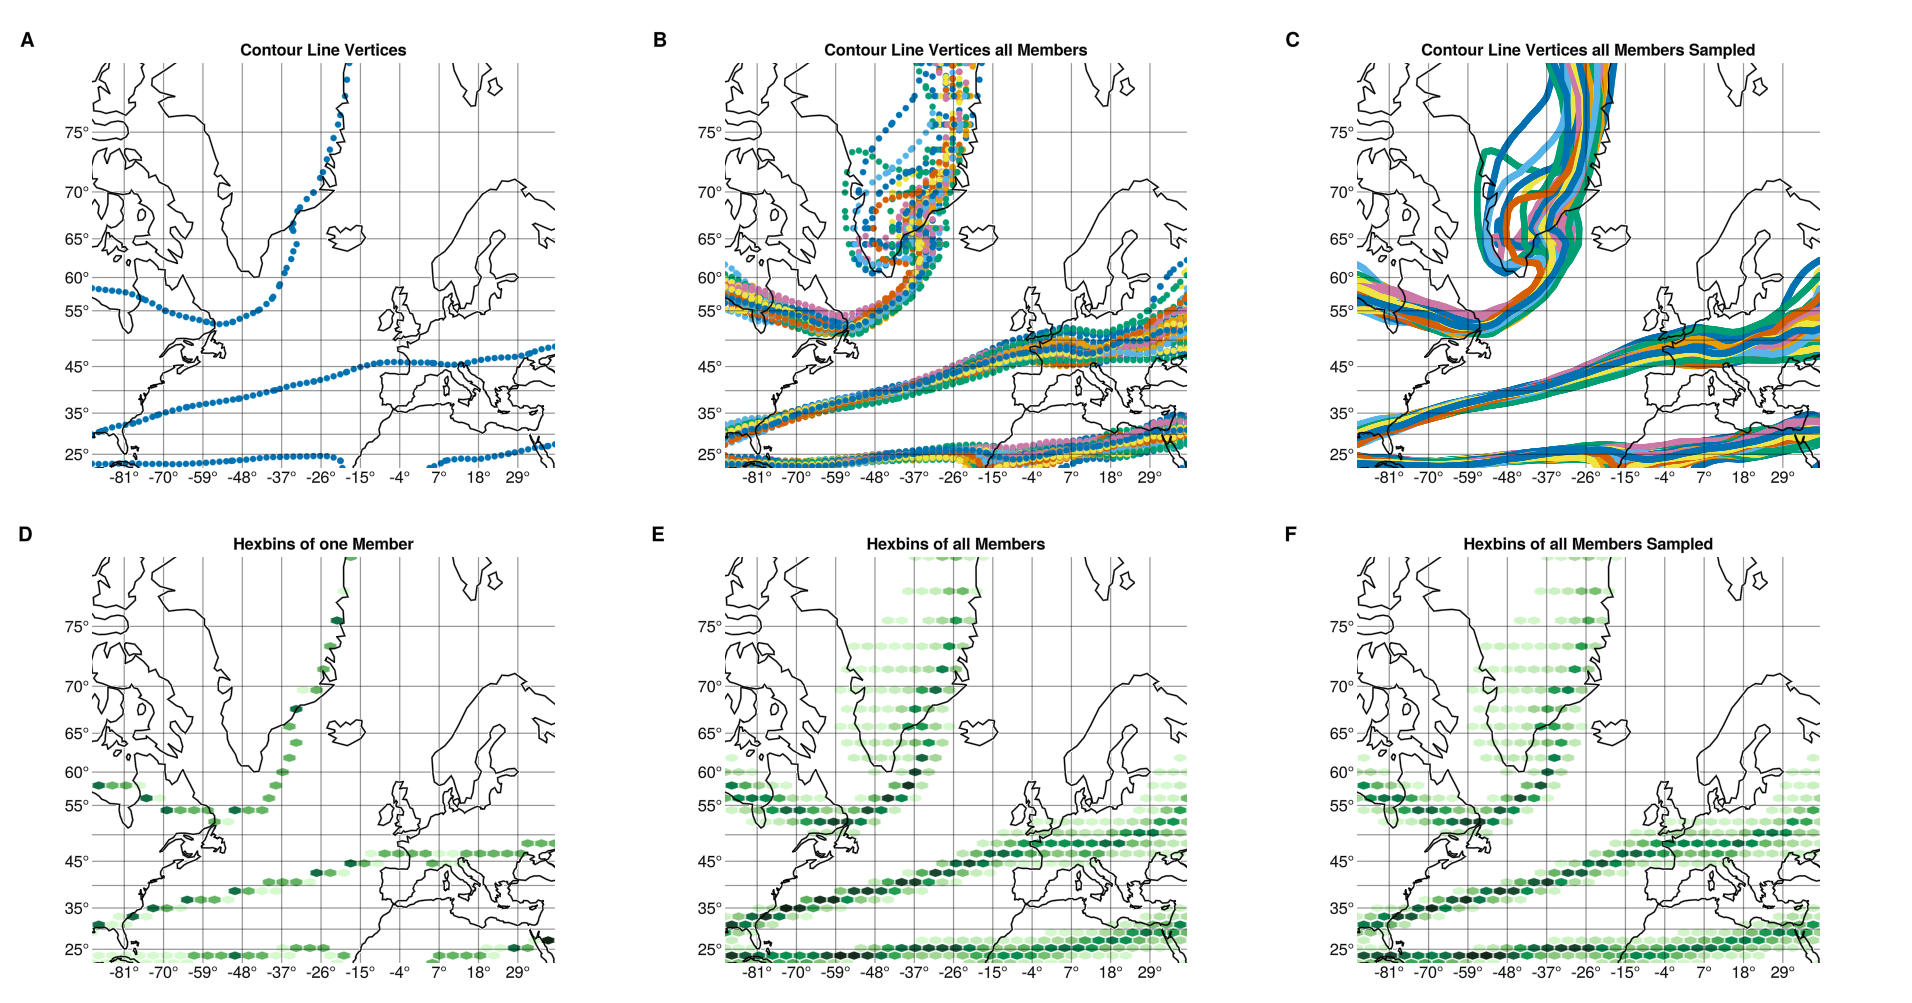
\includegraphics[width=0.95\textwidth]{figures/hexbin_approach_overview.png}
  \end{center}
  \caption{Example of the hexbin approach using the dominant IVT pattern. Sample distance is $0.1$. A to C show the contour lines vertices in one member, all members and all members with sampling along the line. D to F show the hexbin visualization of the corresponding vertices.}\label{fig:hexbin overview}
\end{figure}


The approach using hexbins was conducted as follows: First, the required contour lines were computed, which are represented as a list of 2D points. 
The threshold for displayed hexbins was set to one, so that areas without any contour line stay free of hexagons. 
Since the resolution is too high at some places (multiple observations per bin) and too low at others (no observation hitting the bin) like it is depicted in Figure~\ref{fig:hexbin overview} A and D, a sampling algorithm  was used to sample along the line. 
Of course this results in a distorted color bar since one observation, but by choosing a small enough integration distance (i.e. $0.01$), this distortion is reduced to an invisible minimum. 
So now by using multiple members (Figure~\ref{fig:hexbin overview}, E and F), it approximates the number of lines hitting a certain bin. 
An analysis comparing this approach to the traditional spaghetti plots is given in Section~\ref{sec:pattern evolution}. 

% \begin{itemize}
%   \item greates challenge comes from the variability introduced by the multiple members of the dataset. 
%   \item vizualizing the scalar data turns the 2D map into a 3D cube. 
%   \item there are multiple ways of handling this: either plot a 3D object encoding the variability in the third dimension, or by using the noise technique from \citeauthorwork{coninx_visualization_2011} or by using isocontours. 
%   \item Since the most dominant patterns of IVT show very clear seperation between positive and negative patterns (see Figure TODO), the method of level-crossing probabilities \cite{poethkow_approximate_2013} was implemented.  
%   \item The level set of switching was chosen to be 0, which means that the contours indicate the borders of negative/positive patterns.  \item Those show the borders in scalar fields
% \end{itemize}


\subsection{Temporal Pattern Correlation} % (fold)
\label{sec:Temporal Pattern Correlation}

The spatial pattern is of course only the half of the EOFs. 
An equally important part are the EOF coefficients, representing the activity of the spatial patterns in each (monthly) time step. 
Unfortunately, it is very hard to visualize them on ensemble scale, since each member is quite different in each month, resulting in a hard to interpret mess when using mean functions or boxplots. 

So instead the temporal activity can either a) be analyzed on its own using standard deviation or b) it can be used to evaluate the relationship of certain patterns with other variables or even other patterns. 
For the former it is important to scale the EOF coefficients with the singular values, since on their own they have a standard deviation of one. 
The standard deviation of the scaled EOFs is then calculated for each sliding window and member and visualized using boxplots. 

For the latter, it is very important that the same members are compared across variables since they share their initial conditions and forcings.  
The tool of choice for comparing the temporal patterns/signals is (cross)correlation, which measures the linear relation between two signals. 
This does not imply any causality in any direction on itself, but shows how similar signals (e.g. the EOF coefficients) are. 
Causality must therefor be justified separately from correlation.  
Cross-correlation measures the correlation between two signals with a pre-defined range of lags (e.g. $-n,\dots,0,\dots,n$) to find correlations which are shifted in time. 
A lag of zero is then equal to the usual, non-shifted correlation. 

\subsubsection{Comparing two EOF patterns}

To explore the relationships between certain patterns, the EOF coefficients can be compared to the EOF coefficients of another variable. 
This can answer the question of which patterns share activity in a certain month and how this relationship evolves over time. 

This is evaluated using cross-correlation. 
The reason for this was that introducing a lag to the signal, it could reveal certain temporal relationships, e.g. a positive IVT EOF coefficient of EOF2 (see Figure~\ref{fig:5modes each variable}) leads to positive activity of the precipitation pattern positive in Great Britain (e.g. PR EOF2). 

This evaluation was conducted in the following way: 
Per scope (30 or 50 winters), the cross-correlation of two different variables $X$ and $Y$ was calculated for two modes $a$ and $b$ by calculating the cross-correlation of their temporal patterns $c_a^X(t)$ and $c_b^Y(t)$. 
The range of lags used was $[-n,n] \in \mathbb{Z}$, $n$ being the half of the scopes' length. 
Of course a greater extend of lag could be chosen, but it seemed very unlikely that moisture transport in a certain month would affect precipitation a many decades later (same reasoning for the other variables).
Then the maximal extend of correlation per member was used for a boxplot of that scope.
The lag associated with that value per member was then displazed in a separate boxplot of lags. 
Then this procedure was repeated for every scope from the begin of the historical simulation to the end of each scenario, depicting the evolution over time. 

Since only the temporal coefficients (without the spatial patterns) are evaluated here, it is crucial that the alignment of the patterns (as described in Section~\ref{sec:mode_alignment}) works well since it can distort the correlation results significantly. 
In fact, using this kind of analysis revealed the lack of stability of the procedure used by \citeauthorwork{vietinghoff_visual_2021} in EOF2 and lesser modes. 
For this the plots of the maximal absolute value of correlation were compared to the normal maximal extend of correlation. 
If the plot of absolute correlation revealed a consistently high value, but the normal correlation fluctuated around zero (or had many outliers mirrored on the x-axis), the alignment of patterns did not work correctly. \todo{Example Picture?}


\subsubsection{Comparing an EOF pattern with another variable}

Since it is notoriously hard to connect (mathematical) EOF modes to real physical modes \cite{hannachi_empirical_2007, dommenget_cautionary_2002}, it is not enough to analyze the relationships between patterns since they may not represent any actual physical modes (see the simple example explained in \citeauthorwork{dommenget_cautionary_2002}). 
Instead, the recommendations of \citeauthorwork{dommenget_cautionary_2002} were followed, using different statistical tools to evaluate the modes. 
Some of the related work \cite{zou_interdecadal_2018, zhou_atmospheric_2005, li_quasi-4-yr_2012} used regression maps, depicting the regression slopes between the EOF coefficient $c_a^X(t)$ of variable $X$ and mode $a$ (e.g. the dominant EOF mode of IVT $c_1^{IVT}(t)$)and the temporal evolution of each gridpoints $Y(lon, lat)(t)$ of another variable $Y$. 
\citeauthorwork{fernandez_analysis_2003} used a similar procedure but with the correlation of $c_a^X(t)$ and $X(lon, lat)(t)$, so depicting the correlation coefficient for each gridpoint with the temporal pattern for the same variable $X$. 
This tackles the problem described by \citeauthor{dommenget_cautionary_2002}: \enquote{The PCs of the dominant patterns are often a superposition of many different modes that are uncorrelated in time and that are often modes of remote regions that have no influence on the region in which the pattern of this PC has its center of action.} \cite{dommenget_cautionary_2002} 


For this Thesis an interactive comparison of the patterns of any variable $X$ and the actual data of another (or the same) variable $Y$ was implemented.
To display the ambiguity introduced by the different members, spaghetti plots and the hexbin approach described above were reused, highlighting contour lines of certain correlation levels. 
Therefor, they display areas with correlation higher (or lower) then an interactively chosen correlation level (e.g. $0.7$). 
Also, the mode and the scope can be interactively chosen, to explore different modes and their evolution in time. 
Of particular interest are here the correlation between IVT modes and precipitation data, which could help to explain how the dominant IVT modes influence the precipitation in Europe. 

% section Temporal Pattern Correlation (end)
%
% \subsection{Scenario Comparison} % (fold)
% \label{sec:Scenario Comparison}
%
% \begin{itemize}
%   \item To compare certain scenarios, a interactive visualization was implented. 
%   \item this allows switching data of scenarios on and off (either the boxplots of the temporal analysis as well as correlation maps and level crossing probabilities visualization)
% \end{itemize}
%
% section Scenario Comparison (end)


